% --- Tensor (intra-layer) parallelism ---
\begin{frame}{Tensor Parallelism: Split the Matrix, Not the Batch}
  \begin{itemize}\footnotesize\itemsep0.35em
    \item[\textcolor{red}{$\blacktriangleright$}] Every technique so far kept whole layers on one device. \textbf{Tensor parallelism} cuts \emph{inside} a layer, so a single weight matrix lives on $t$ GPUs at once. It is the only tool that helps when one layer alone exceeds one device.
    \item[\textcolor{red}{$\blacktriangleright$}] There are exactly two ways to split a matrix multiply $Y = XA$, and Megatron-LM's contribution is choosing the right one at each position so the two compose with no communication in between.
    \item[\textcolor{red}{$\blacktriangleright$}] \textbf{Column-parallel.} Split $A = [A_1, A_2]$ by columns; each rank computes $XA_i$ from a replicated $X$ and holds a slice of the output, $[Y_1, Y_2] = [XA_1,\; XA_2]$. Any \emph{elementwise} nonlinearity then applies independently to each slice --- $\mathrm{GeLU}(XA_i)$ is exactly the matching slice of $\mathrm{GeLU}(XA)$ --- so nothing needs to be exchanged.
    \item[\textcolor{red}{$\blacktriangleright$}] \textbf{Row-parallel.} Split $B = [B_1; B_2]$ by rows and feed it the already-split $Y$. Each rank now computes a \emph{partial sum} of the full output:
      \[
        Z = YB = Y_1B_1 + Y_2B_2 \quad\Longrightarrow\quad \text{one all-reduce to finish.}
      \]
    \item[\textcolor{red}{$\blacktriangleright$}] Chain them --- column-parallel, then row-parallel --- and a two-matrix block costs \textbf{one} all-reduce instead of two. This is why the split must respect the nonlinearity: splitting $A$ by rows instead would force a synchronisation before the GeLU.
  \end{itemize}
\end{frame}

\begin{frame}{The MLP Block}
  \centering
  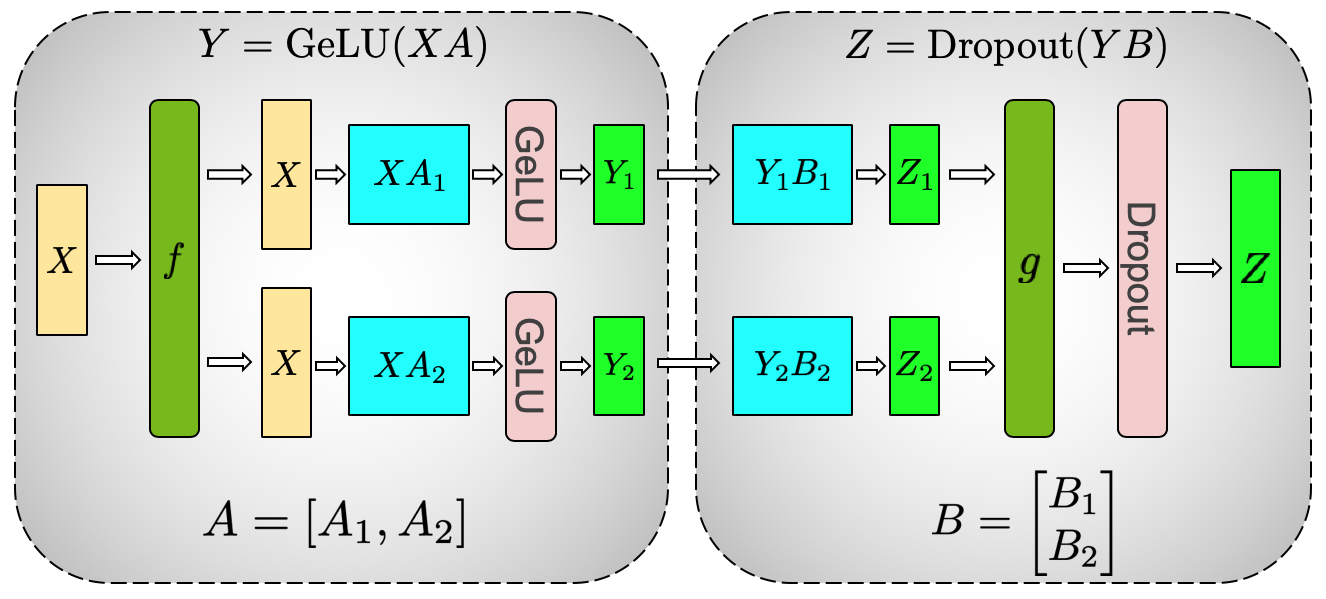
\includegraphics[width=0.8\textwidth,height=0.5\textheight,keepaspectratio]{images/distributed-training/megatron_fig3a_mlp_tensor_parallel.png}\\[0.3em]
  \begin{itemize}\scriptsize\itemsep0.05em
    \item[\textcolor{red}{$\blacktriangleright$}] $f$ and $g$ are \textbf{conjugate} operators: $f$ is the identity in the forward pass and an all-reduce in the backward pass; $g$ is an all-reduce in the forward pass and the identity in the backward pass.
    \item[\textcolor{red}{$\blacktriangleright$}] So the whole MLP block costs \textbf{one all-reduce forward and one backward}, and the GeLU in the middle is free.
    \item[\textcolor{red}{$\blacktriangleright$}] Note what is \emph{not} split: the input $X$ and output $Z$ are replicated on every rank. Tensor parallelism shards the weights and the intermediate activations, not the block boundaries.
  \end{itemize}
  \vspace{0.03em}
  {\scriptsize Shoeybi et al., ``Megatron-LM: Training Multi-Billion Parameter Language Models Using Model Parallelism,'' \href{https://arxiv.org/abs/1909.08053v4}{arXiv:1909.08053v4}, Figure 3(a).}
\end{frame}

\begin{frame}{Self-Attention: Sharding Falls Out of the Architecture}
  \begin{columns}[T,onlytextwidth]
    \column{0.5\textwidth}
      \begin{itemize}\footnotesize\itemsep0.3em
        \item[\textcolor{red}{$\blacktriangleright$}] Multi-head attention is \emph{already} a sum over independent heads, so the split needs no new idea: give each rank a disjoint subset of heads.
        \item[\textcolor{red}{$\blacktriangleright$}] The $Q$, $K$, $V$ projections are \textbf{column-parallel}; the output projection is \textbf{row-parallel}. Result: one all-reduce forward, one backward, and the softmax --- the expensive part --- never crosses a device boundary.
        \item[\textcolor{red}{$\blacktriangleright$}] \textbf{Divisibility constraints} bite in practice: $t$ must divide the number of attention heads, the hidden size, and the MLP intermediate size. With grouped-query attention it must also divide the number of \emph{key/value} heads --- often only 8, which caps $t$ at 8.
        \item[\textcolor{red}{$\blacktriangleright$}] Embedding and output layers get a \textbf{vocabulary-parallel} split with a fused cross-entropy, avoiding an all-gather of the full logits.
      \end{itemize}
    \column{0.48\textwidth}
      \centering
      \vspace{0.3em}
      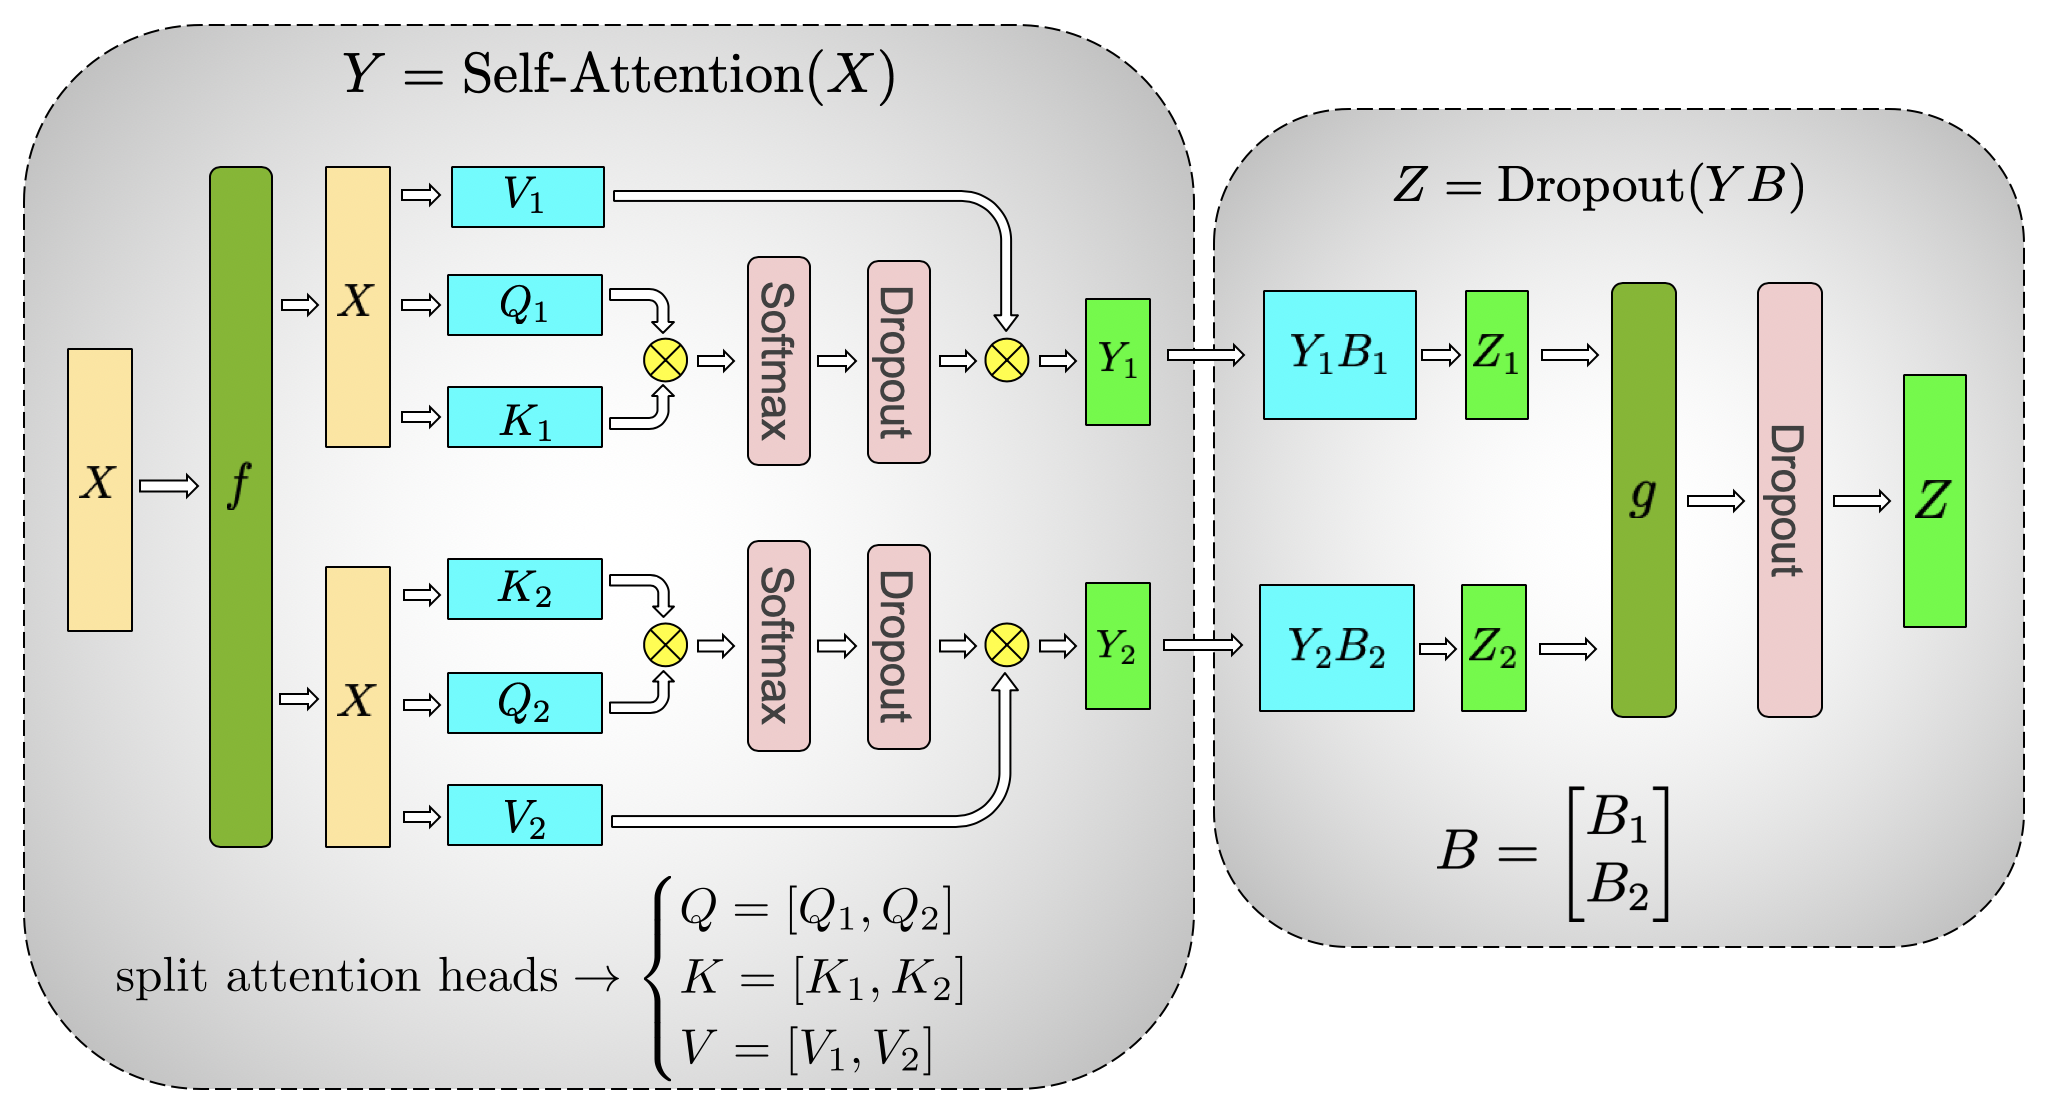
\includegraphics[width=\linewidth,height=0.66\textheight,keepaspectratio]{images/distributed-training/megatron_fig3b_attention_tensor_parallel.png}\\[0.2em]
      {\scriptsize Shoeybi et al., \href{https://arxiv.org/abs/1909.08053v4}{arXiv:1909.08053v4}, Figure 3(b).}
  \end{columns}
\end{frame}

\begin{frame}{The Communication Bill}
  \begin{columns}[T,onlytextwidth]
    \column{0.46\textwidth}
      \centering
      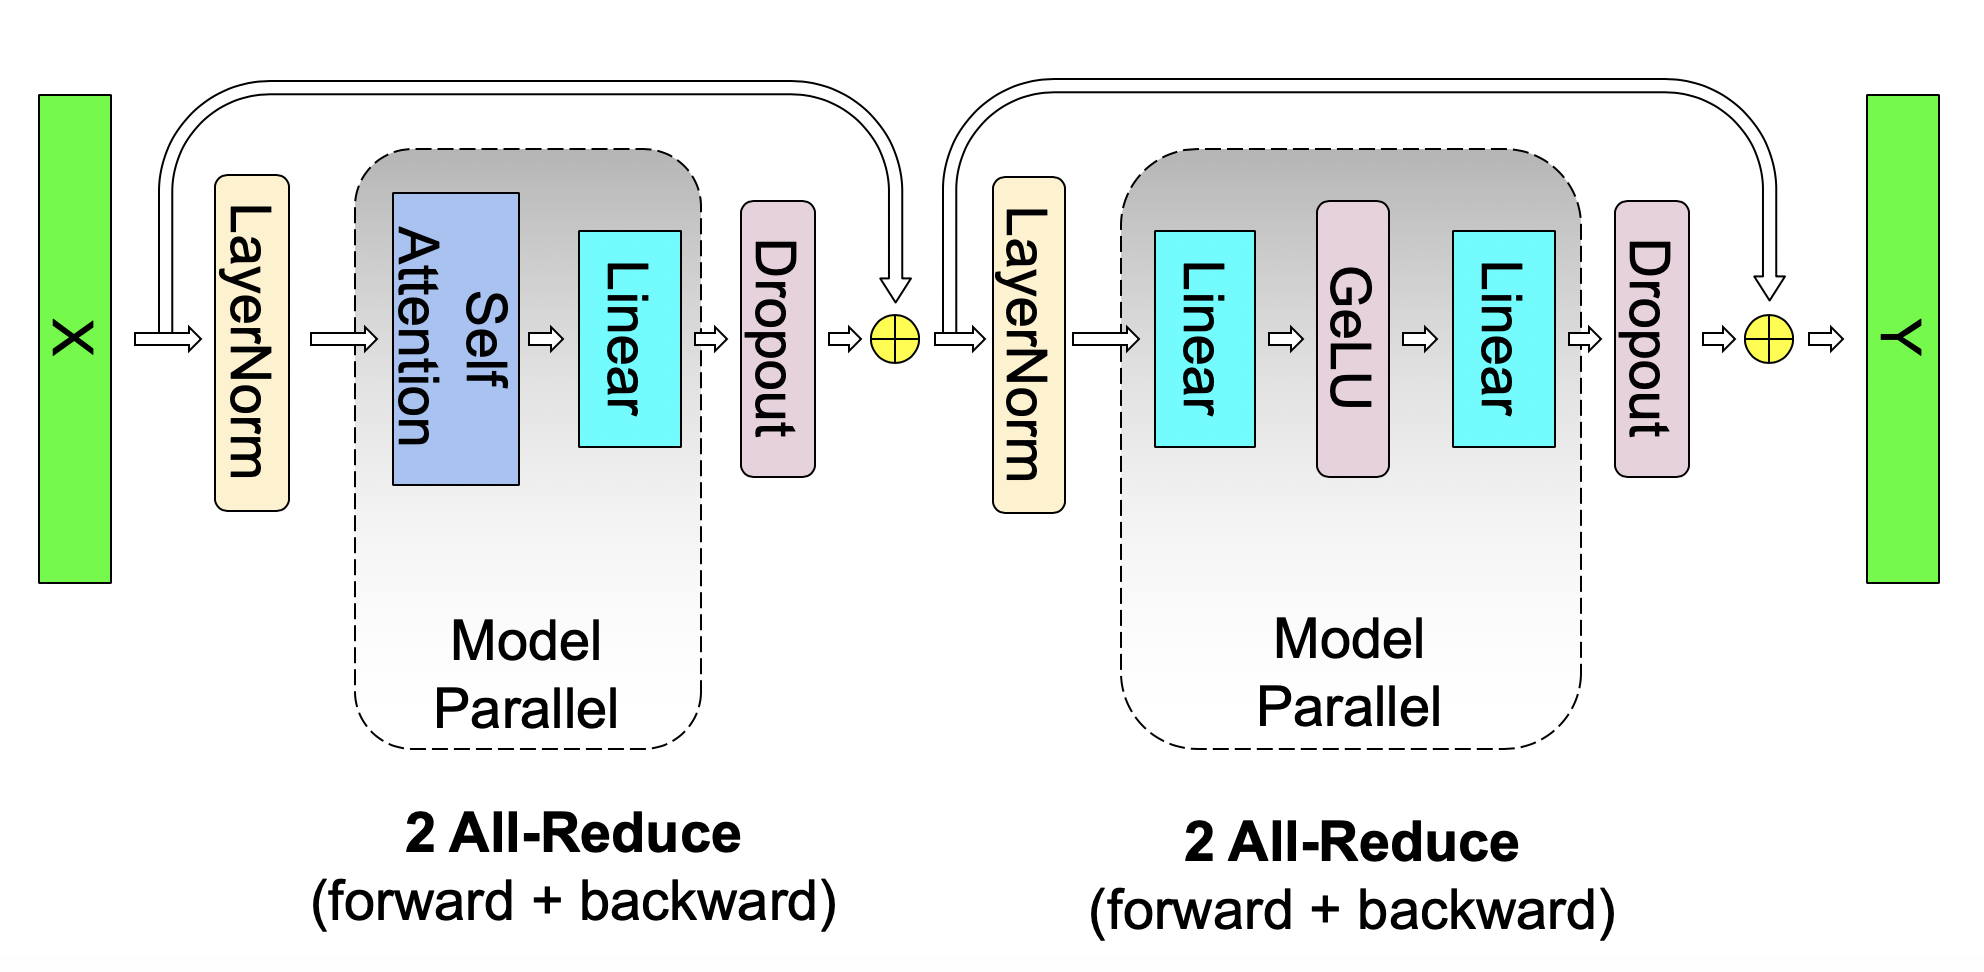
\includegraphics[width=\linewidth,height=0.58\textheight,keepaspectratio]{images/distributed-training/megatron_fig4_communication_operations.png}\\[0.2em]
      {\scriptsize Four all-reduces per transformer layer per iteration. Shoeybi et al., \href{https://arxiv.org/abs/1909.08053v4}{arXiv:1909.08053v4}, Figure 4.}
    \column{0.52\textwidth}
      \begin{itemize}\footnotesize\itemsep0.3em
        \item[\textcolor{red}{$\blacktriangleright$}] Two all-reduces forward (one per block) and two backward: \textbf{four per layer, per iteration}, each on a tensor of $b \cdot s \cdot h$ elements. Full activation recomputation reruns the forward pass, making it six.
        \item[\textcolor{red}{$\blacktriangleright$}] Since an all-reduce moves $\approx 2\times$ the message size per rank, the traffic per layer per iteration is about $8\,b\,s\,h$ elements. For a 7B-class model ($h = 4096$, $L = 32$) at $b = 4$, $s = 2048$ in \texttt{bf16}, that is $\approx 17$\,GB per GPU per step.
        \item[\textcolor{red}{$\blacktriangleright$}] \textbf{The volume is not the problem --- the placement is.} Data-parallel traffic happens once, at the end of the backward pass, and DDP hides it behind computation. Tensor-parallel traffic sits \textbf{on the critical path}: the next operation literally cannot start until the all-reduce lands.
        \item[\textcolor{red}{$\blacktriangleright$}] The compensation is that tensor parallelism shards \emph{activations} too, so it reduces the memory term that ZeRO cannot touch.
      \end{itemize}
  \end{columns}
\end{frame}

\begin{frame}[allowframebreaks]{Why Tensor Parallelism Stays Inside a Node}
  \begin{itemize}\itemsep0.4em
    \item[\textcolor{red}{$\blacktriangleright$}] Put the two facts together. Tensor-parallel collectives are (i) frequent --- four per layer, so 128 per iteration for a 32-layer model --- and (ii) unhideable, because they are synchronisation points in the middle of a layer.
    \item[\textcolor{red}{$\blacktriangleright$}] Now compare the two fabrics they might run over. An H100 SXM has \textbf{900\,GB/s} of NVLink bandwidth to its neighbours through NVSwitch. A single NDR InfiniBand port gives \textbf{50\,GB/s}. That is an \textbf{18$\times$} gap on traffic you cannot overlap.
    \item[\textcolor{red}{$\blacktriangleright$}] Hence the standard rule, stated as Takeaway \#1 by Narayanan et al.:
      \begin{itemize}
        \item[] \footnotesize\textit{``When considering different forms of model parallelism, tensor model parallelism should generally be used up to degree $g$ when using $g$-GPU servers, and then pipeline model parallelism can be used to scale up to larger models across servers.''}
      \end{itemize}
    \item[\textcolor{red}{$\blacktriangleright$}] In practice this means \textbf{$t \leq 8$} on an 8-GPU HGX node, and the same rule reappears verbatim in inference serving: vLLM's guidance is to set tensor-parallel size to the GPUs per node and pipeline-parallel size to the number of nodes.
    \item[\textcolor{red}{$\blacktriangleright$}] Tensor parallelism also \emph{shrinks} the per-GPU batch, since the batch is replicated across the tensor-parallel group. Pushing $t$ too high starves the GEMMs and drops utilisation even if the bandwidth were free.
  \end{itemize}
  \vspace{0.1em}
  {\scriptsize Narayanan et al., ``Efficient Large-Scale Language Model Training on GPU
  Clusters Using Megatron-LM,'' SC 2021.
  \href{https://arxiv.org/abs/2104.04473v5}{arXiv:2104.04473v5}, Section 3.2.}
\end{frame}
